Aunque BGP fue diseñado originalmente para el intercambio de rutas IPv4, la arquitectura de Internet ha evolucionado hacia un entorno multiprotocolo. La necesidad de soportar nuevas tecnologías como \textbf{IPv6} y \textbf{MPLS} llevó al desarrollo de extensiones que permiten a BGP actuar como un transporte universal de información de alcanzabilidad.

\subsection{MPLS y el Enrutamiento Basado en Etiquetas}

\textbf{MPLS (\textit{Multi-Protocol Label Switching})} es una tecnología de conmutación que permite dirigir paquetes a través de una red utilizando "etiquetas" cortas en lugar de realizar búsquedas complejas en tablas de direcciones de red extensas. Estas etiquetas se insertan entre las capas 2 y 3 del modelo OSI, permitiendo una conmutación extremadamente rápida y la creación de redes privadas virtuales (VPN) y túneles de ingeniería de tráfico. BGP juega un papel fundamental al distribuir las etiquetas necesarias para que los enrutadores MPLS sepan cómo conmutar el tráfico hacia los destinos remotos.

\subsection{BGP Multiprotocolo (MP-BGP)}

Para evitar el desarrollo de un protocolo nuevo para cada tecnología, el IETF introdujo las extensiones \textbf{MP-BGP}. Estas permiten que una única sesión BGP transporte múltiples "familias de direcciones" (AFI) de forma simultánea y aislada.

La innovación clave es el concepto de \textbf{NLRI (\textit{Network Layer Reachability Information})}. Tradicionalmente, un anuncio BGP era solo un prefijo IPv4. Con NLRI, el concepto se generaliza: la "Información de Alcanzabilidad" puede ser un prefijo IPv6, una etiqueta MPLS, o incluso información de VPN.

\subsection{Atributos NLRI: MP\_REACH y MP\_UNREACH}

Las extensiones se transportan mediante dos nuevos atributos de ruta que sustituyen la sección tradicional de destinos del mensaje UPDATE:

\begin{itemize}
	\item \textbf{MP\_REACH\_NLRI (Tipo 14):} Se utiliza para anunciar destinos alcanzables de cualquier familia de direcciones (IPv6, MPLS, etc.). Incluye la dirección del \textit{Next-Hop} adaptada al protocolo correspondiente y la lista de destinos específicos.
	\item \textbf{MP\_UNREACH\_NLRI (Tipo 15):} Informa sobre destinos que han dejado de ser alcanzables para una familia de direcciones específica.
\end{itemize}

\begin{figure}[H]
	\centering
	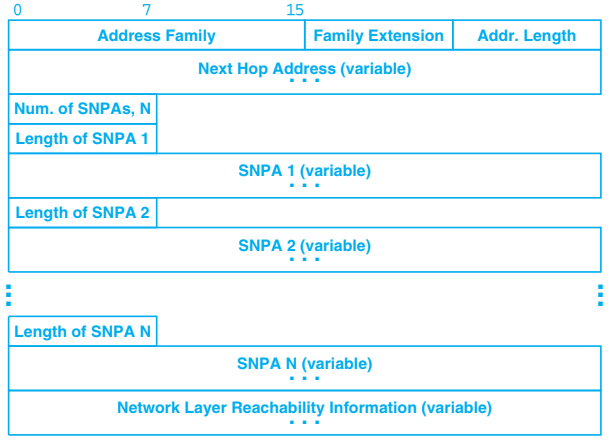
\includegraphics[width=0.8\textwidth]{img/NLRI_atributos.png}
	\caption{Estructura del atributo MP\_REACH\_NLRI para soporte multiprotocolo.}
	\label{fig:grafico9}
\end{figure}

Estos atributos son \textbf{opcionales} (permitiendo compatibilidad con enrutadores antiguos) y \textbf{no transitivos} (asegurando que solo los enrutadores explícitamente configurados para una familia de direcciones procesen dicha información).

\subsection{Economía del Enrutamiento en Internet}

En el núcleo de Internet, las decisiones de BGP no están dictadas por el rendimiento técnico, sino por acuerdos comerciales entre Proveedores de Servicios de Internet (ISP). Estos acuerdos se dividen principalmente en tres categorías:

\begin{itemize}
	\item \textbf{Relación Cliente-Proveedor:} Un ISP pequeño paga a uno más grande (Tier-1 o Tier-2) por el acceso a la tabla de rutas global. El tráfico que fluye hacia el proveedor genera costos para el cliente.
	\item \textbf{Acuerdos de Peering (Pares):} Dos ISP de jerarquía similar intercambian tráfico de sus respectivos clientes de forma gratuita o con costos compartidos. Este acuerdo es mutuamente beneficioso pero requiere un equilibrio en el volumen de datos intercambiados.
	\item \textbf{Tránsito:} Un acuerdo donde un ISP permite que el tráfico de un tercero atraviese su red para llegar a otros destinos, cobrando generalmente por este servicio.
\end{itemize}

\subsubsection{Manipulación de BGP por Incentivos Económicos}

Un ISP configurará sus políticas BGP para priorizar las rutas que le generen ingresos. Por ejemplo, siempre preferirá una ruta a través de un \textbf{Cliente} (donde cobra por bit) que a través de un \textbf{Proveedor} (donde paga por bit), incluso si la ruta del proveedor es técnicamente más corta.

Para evitar el tráfico no deseado o costoso, los administradores emplean técnicas de manipulación como el \textbf{AS-PATH Prepending}: añadir artificialmente el propio número de AS varias veces en un anuncio para que la ruta parezca "más larga" ante los vecinos y así disuadirlos de usarla, forzando el tráfico por caminos económicamente más favorables.
